
\begin{figure}[ht]
\centering

\begin{subfigure}[b]{0.45\textwidth}
    \centering
    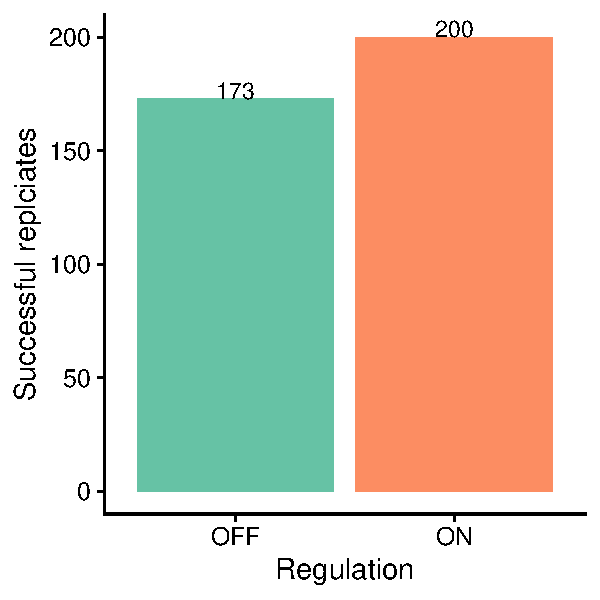
\includegraphics[width=\linewidth]{chapters/05-tag-based-genetic-regulation/media/context-signal-solution-counts.pdf}
    \caption{\small Successful replicates.}
    \label{chapter:tag-based-regulation:subfig:context-signal-solution-counts}
\end{subfigure}
\hfill
\begin{subfigure}[b]{0.45\textwidth}
    \centering
    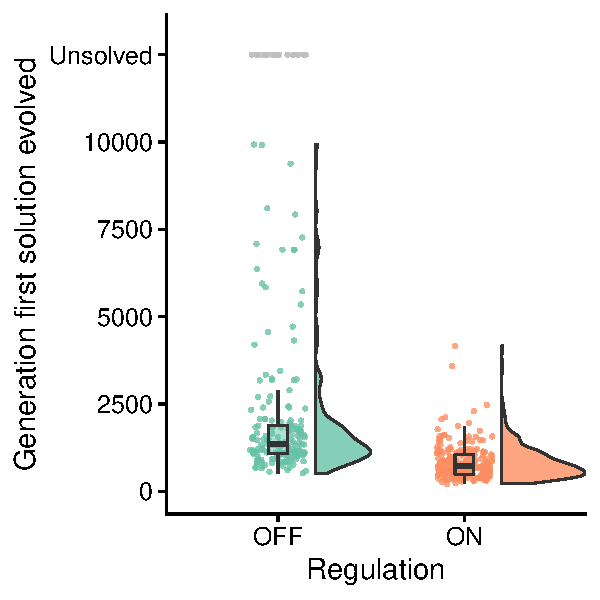
\includegraphics[width=\textwidth]{chapters/05-tag-based-genetic-regulation/media/context-signal-solve-time-cloud.pdf}
    \caption{\small Generations elapsed before solution.}
    \label{chapter:tag-based-regulation:subfig:context-signal-solve-time}
\end{subfigure}

\caption{\small 
\textbf{Contextual-signal problem-solving performance.}
(a) shows the number of successful replicates for the regulation-off and regulation-on conditions on the contextual-signal problem. 
The regulation-off condition was less successful than the regulation-on condition (Fisher's exact test: $p < 6\times10^{-9}$).
(b) is a raincloud plot showing the generation at which the first solution evolved in each successful replicate.
Gray points indicate the number of unsuccessful replicates for each condition.
Regulation-on solutions typically required fewer generations than regulation-off solutions to arise  (Wilcoxon rank sum test: $p < 10^{-15}$).
}

% problem-solving success - p-value = 5.818e-09; fisher's
% solve time: p-value < 2.2e-16; wilcoxon
    
\label{chapter:tag-based-regulation:fig:context-signal-performance}
\end{figure}
